%%%% SIGNAL SECTION %%%%
\section{MCS Performance on Muons from numuCC Events in MicroBooNE Data}\label{data_performance_section}

\subsection{Input sample}
reference CCInclusive technote, good runs list, no EXT data used only BNB. cosmic backgrounds are low after event selection (quantify this probably). especially low after hand scanning too

\subsection{Event selection}
\begin{enumerate}
\item describe the event selection, 2 tracks at vertex, etc etc.
\item state we take tracks fully contained in fiducial volume, longer than 1 meter
\item state that broken tracks and MIDs are still present so we do hand scanning
\item describe hand scanning, include pictures of event displays like Figure \ref{bad_evd_fig_1}.
\item numbers: from 5e19 POT ended up with X events, of those 598 have the fully contained longer than 1 meter track, and 396 are deemed well-reconstructed after handscanning.
\end{enumerate}


\begin{figure}[h!]
\begin{center}
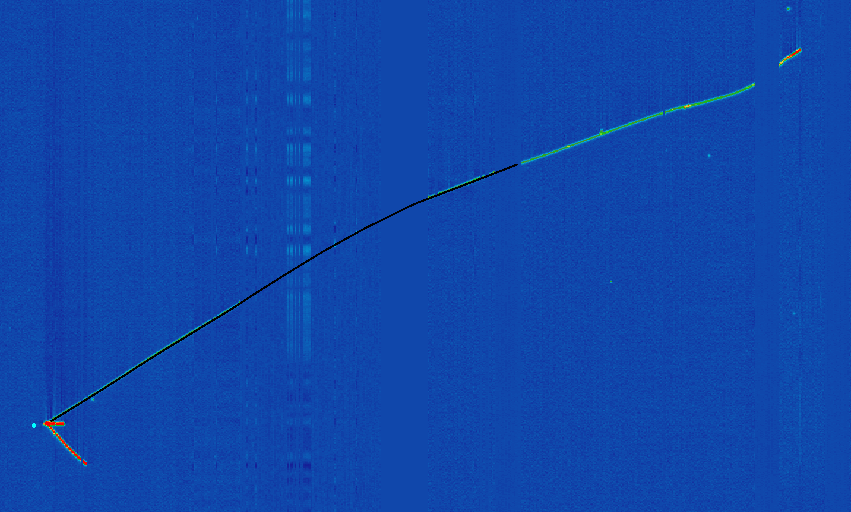
\includegraphics[width=100mm]{Figures/bad_evd_1.png}
\end{center}
\caption{\textit{bad evd caption}}
\label{bad_evd_fig_1}
\end{figure}

\subsection{MCS Energy Validation}\label{MCS_Energy_Validation_DataRecoTrack_section}
For this sample of reconstructed tracks, the trajectory points only of each track is used as input to the MCS code, described in Section XXX. The resulting MCS energy versus range-based energy without any additional hand-scan reconstruction quality checks can be seen in Figure \ref{MCS_range_energy_DataRecoTrack_nohandscan_fig}. The off-diagonal visible in this figure (where MCS energy greatly overestimates range energy) is caused by poor track reconstruction (truncated tracks) and MIDs. Figure \ref{MCS_range_energy_RecoTrack_withandwithouthandscan_fig} divides Figure \ref{MCS_range_energy_DataRecoTrack_nohandscan_fig} into those events which are handscanned as having poorly reconstructed or obviously MID'd tracks, and those which are well reconstructed. It can be seen that hand-scanning tends to remove the off-diagonal and therefore improve the MCS energy resolution.\\

In order to compute a bias and a resolution, Figure \ref{MCS_range_energy_DataRecoTrack_fig} is sliced in bins of range energy and a histogram of the fractional energy difference ($\frac{E_{MCS} - E_{range}}{E_{range}}$) is created for each bin. This distribution is shown for two representative bins in Figure \ref{MCS_range_bias_resolution_DataRecoTrack_slices_fig}. The mean of each distribution is used to compute a bias a function of range, while the standard deviation of each distribution is used to compute a resolution. The bias and resolution for this energy reconstruction method shown in Figure \ref{MCS_range_bias_resolution_DataRecoTrack_fig}. This figure indicates a bias in the MCS energy resolution on the order of a few percent, with a resolution that decreases from about 18\% for contained {\sc MCTracks} with true total energy around 0.5 GeV (which corresponds to a length of about 1.7 meters) to below 10\% for contained {\sc MCTracks} with true total energy greater than 0.8 GeV (which corresponds to a length of about 3.1 meters). This agrees well with the same bias and resolution measurement in simulation shown in Figure \ref{MCS_range_bias_resolution_MCNuRecoTrack_fig}.


\begin{figure}[h!]
\begin{center}
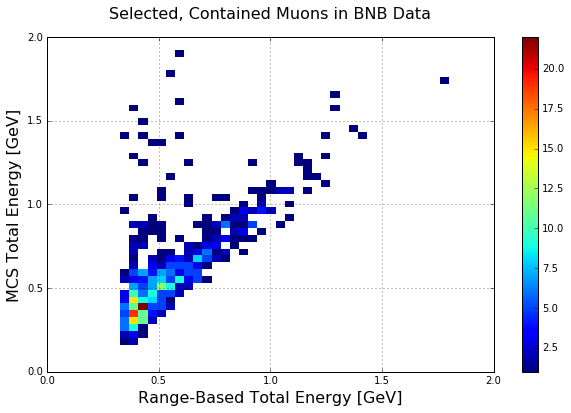
\includegraphics[width=100mm]{Figures/MCS_range_comparison_DataRecoTracks_nohandscan.png}
\end{center}
\caption{\textit{MCS computed energy versus range energy for the selected neutrino-induced fully contained muon sample in data without any additional handscanning to check for reconstruction quality. The off-diagonal where MCS energy greatly overestimates range energy is caused by poor track reconstruction (truncated tracks) and MIDs.}}
\label{MCS_range_energy_DataRecoTrack_nohandscan_fig}
\end{figure}

\begin{figure}
\centering
\mbox{
	\subfigure[\textit{The subset of events in Figure \ref{MCS_range_energy_DataRecoTrack_nohandscan_fig} which were hand-scanned as having poor reconstruction quality or obvious MID topologies.}]
	{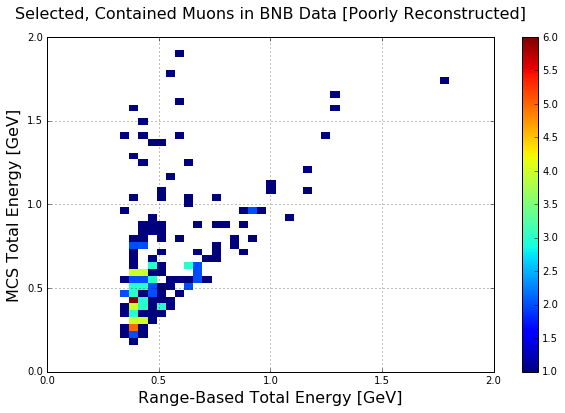
\includegraphics[width=75mm]{Figures/MCS_range_energy_DataRecoTracks_badhandscan.png}}
	\quad
	\subfigure[\textit{The subset of events in Figure \ref{MCS_range_energy_DataRecoTrack_nohandscan_fig} which were hand-scanned as having good reconstruction quality or obvious MID topologies.}\label{MCS_range_energy_DataRecoTrack_fig}]
	{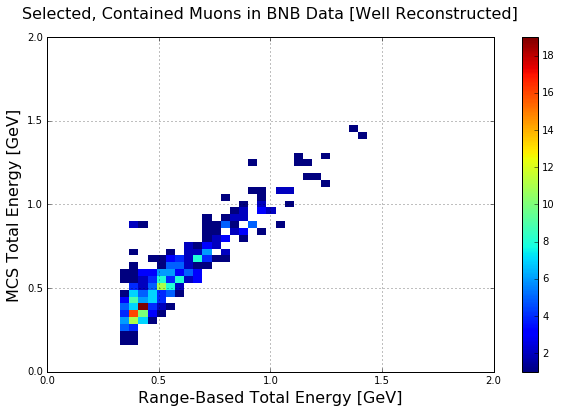
\includegraphics[width=75mm]{Figures/MCS_range_energy_DataRecoTracks_goodhandscan.png}}
	}
\caption{\textit{MCS computed energy versus range energy for the selected neutrino-induced fully contained muon sample in data hand-scanned as having poorly reconstructed tracks (left) and well reconstructed tracks (right).}}
\label{MCS_range_energy_RecoTrack_withandwithouthandscan_fig}
\end{figure}


\begin{figure}
\centering
\mbox{
	\subfigure[\textit{Fractional energy difference between 0.35 and 0.53 GeV range energy.}]
	{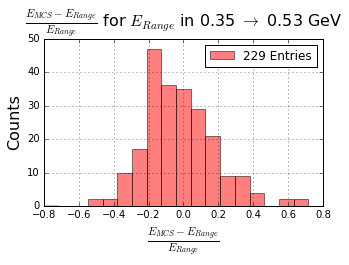
\includegraphics[width=50mm]{Figures/MCS_range_resolution_DataRecoTracks_slice1.png}}
	\quad
	\subfigure[\textit{Fractional energy difference between 0.90 and 1.08 GeV range energy.}]
	{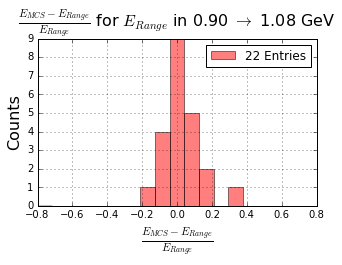
\includegraphics[width=50mm]{Figures/MCS_range_resolution_DataRecoTracks_slice2.png}}
	}
\caption{\textit{Fractional energy difference for a few representative bins of range energy derived from Figure \ref{MCS_range_energy_DataRecoTrack_fig}.}}
\label{MCS_range_bias_resolution_DataRecoTrack_slices_fig}
\end{figure}


\begin{figure}
\centering
\mbox{
	\subfigure[\textit{MCS energy bias as a function of range energy.}]
	{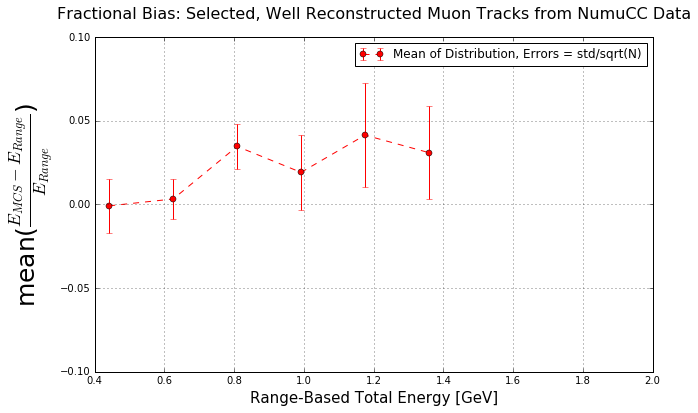
\includegraphics[width=75mm]{Figures/MCS_range_bias_DataRecoTracks.png}}
	\quad
	\subfigure[\textit{MCS energy resolution as a function of range energy.}]
	{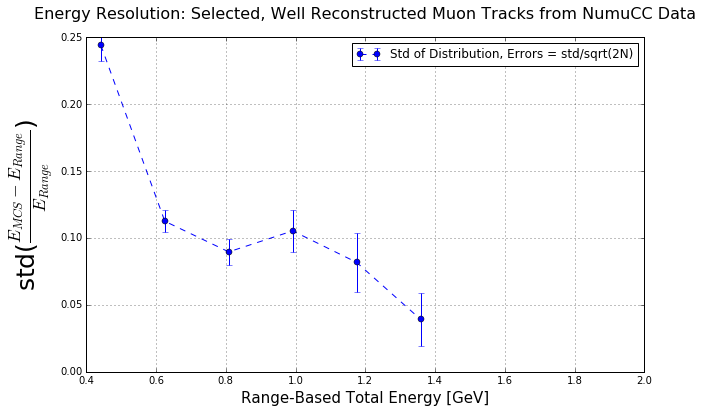
\includegraphics[width=75mm]{Figures/MCS_range_resolution_DataRecoTracks.png}}
	}
\caption{\textit{MCS energy bias and resolution as a function of range energy for the selected, well reconstructed neutrino-induced muons in {\ub} data.}}
\label{MCS_range_bias_resolution_DataRecoTrack_fig}
\end{figure}



\subsection{Highland Validation}\label{Highland_Validation_DataRecoTrack_section}
For a given track segment energy and length, 98\% of the angular scatter deviations should be gaussian with an RMS described by the Highland equation (Equation \ref{highland_eqtn}), while the remaining 2\% are larger angle Rutherford scatters [XXX source]. Therefore, a histogram of track segment angular deviations divided by the RMS predicted by the Highland equation should be gaussian with a width of unity. In this section, we validate this claim.\\

For each 20cm segment of each reconstructed track in this single muon sample, the energy of the muon at the start of that segment is estimated by taking the computed MCS energy and subtracting out energy lost in the track upstream of the start of this segment, assuming the track was minimally ionizing (depositing 2.2 MeV per centimeter of track). This energy, along with the segment length, is converted into an expected RMS angular deviation by way of Equation \ref{highland_eqtn}. For each consecutive pairs of segments, the angular scatter in milliradians divided by the Highland expected RMS in millradians is an entry in the histogram shown in Figure \ref{Highland_validation_DataRecoTracks_fig}. From this figure we can see that the Highland formula is valid for well reconstructed tracks in data.

\begin{figure}[h!]
\begin{center}
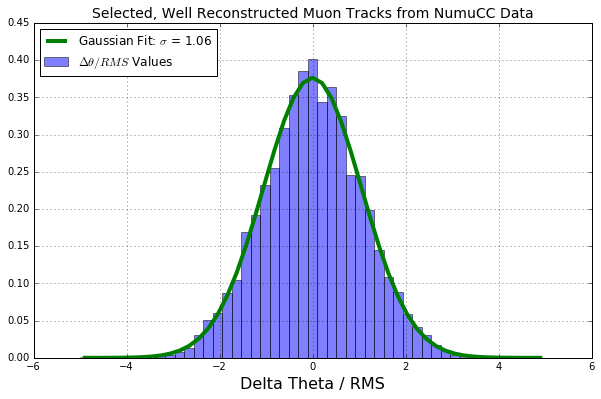
\includegraphics[width=100mm]{Figures/Highland_validation_DataRecoTracks_goodhandscan.png}
\end{center}
\caption{\textit{20cm segment angular deviations divided by expected Highland RMS for the sample of well reconstructed, neutrino induced muons in {\ub} data.}}
\label{Highland_validation_DataRecoTracks_fig}
\end{figure}

\subsection{Optimizing Segment Length}\label{SegmentLength_DataRecoTrack_section}
One of the tunable parameters in the MCS code is the length of segments into which a track is broken. While shorter segment lengths yield more segments per track and therefore more sampling points to build a stronger likelihood, they also lead to the breakdown of the gaussian nature of scatters. Longer segments tend to have more gaussian scatters but lead to fewer sampling points and therefore worse energy resolution. For these two reasons there exists an optimal segment length. Figure \ref{Highland_seglenstudy_DataRecoTracks_fig} shows analogous figures to Figure \ref{Highland_validation_DataRecoTracks_fig} for four different segment lengths ranging between 5cm and 25cm. The input sample for this figure are the neutrino-induced muons that are fully contained and have been deemed well reconstructed. From this figure it can be seen that only segment lengths longer than 20cm provide truly gaussian distributions. Figure \ref{seglenstudy_bias_resolution_DataRecoTrack_fig} shows the bias and resolution for the MCS energy reconstruction method on this same sample. While shorter segment lengths tend to have a slightly higher bias, the difference is small. Similarly, shorter segment lengths tend to have better resolution but the difference is small at larger range energies. For range energies below about 0.5 GeV the difference in resolution between segment lengths grows because the tracks are short enough where the longer segment lengths are not providing enough sampling points for the MCS method to make an accurate estimation of the track energy. In order to maintain a gaussian distribution of angular scatters while providing enough sampling points for an energy resolution of below 30\% for the shortest viable tracks, a segment length of 20cm has been chosen for this analysis.

\begin{figure}
\centering
\mbox{
	\subfigure[\textit{Highland validation figure for 5cm segment lengths.}]
	{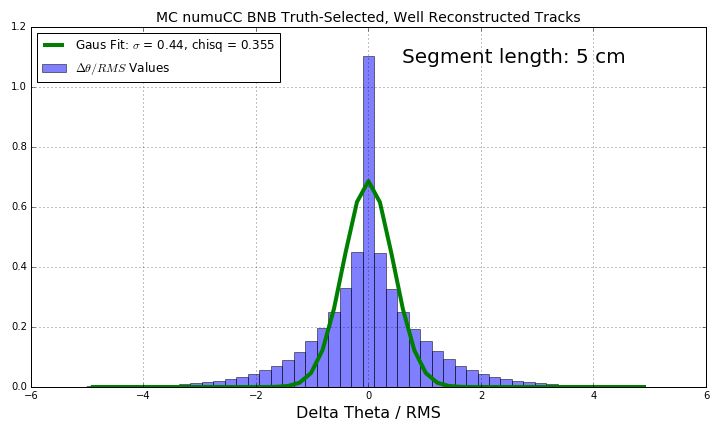
\includegraphics[width=75mm]{Figures/seglenstudy_gaus_5cm.png}}
	\quad
	\subfigure[\textit{Highland validation figure for 10cm segment lengths.}]
	{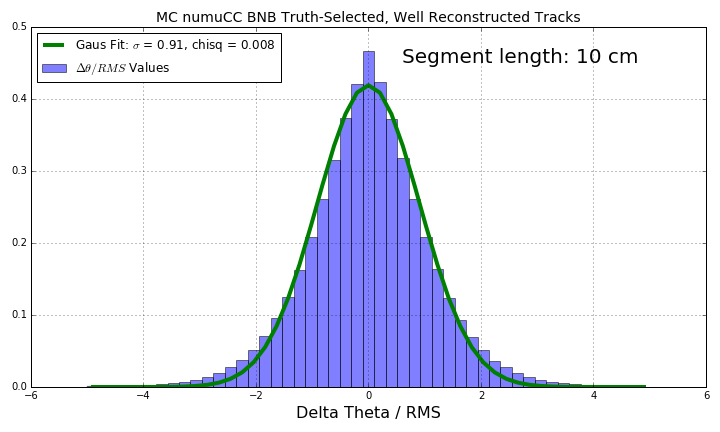
\includegraphics[width=75mm]{Figures/seglenstudy_gaus_10cm.png}}
	}\newline
\mbox{
	\subfigure[\textit{Highland validation figure for 20cm segment lengths.}]
	{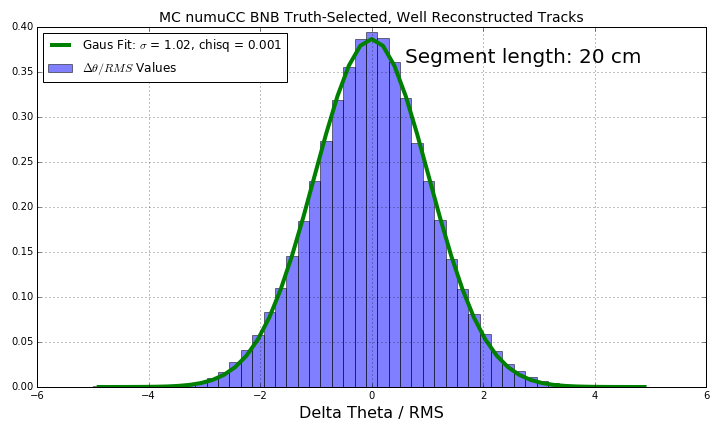
\includegraphics[width=75mm]{Figures/seglenstudy_gaus_20cm.png}}
	\quad
	\subfigure[\textit{Highland validation figure for 25cm segment lengths.}]
	{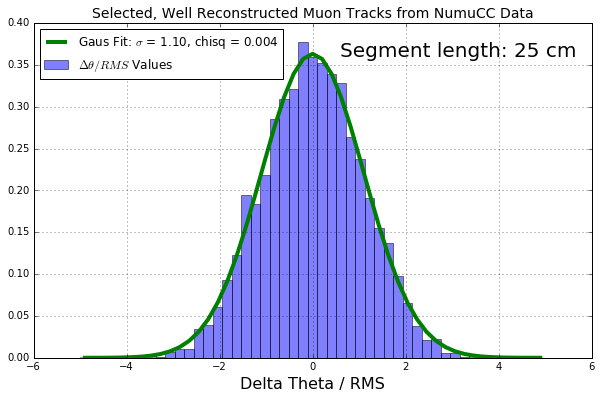
\includegraphics[width=75mm]{Figures/seglenstudy_gaus_25cm.png}}
	}
\caption{\textit{Highland validation figures analogous to Figure \ref{Highland_validation_DataRecoTracks_fig} for various segment lengths, taken from the sample of well reconstructed neutrino-induced muons in {\ub} data. The gaussian nature of this plot breaks down for segment lengths that are too short.}}
\label{Highland_seglenstudy_DataRecoTracks_fig}
\end{figure}



\begin{figure}
\centering
\mbox{
	\subfigure[\textit{MCS energy bias as a function of range energy for four different segment lengths.}]
	{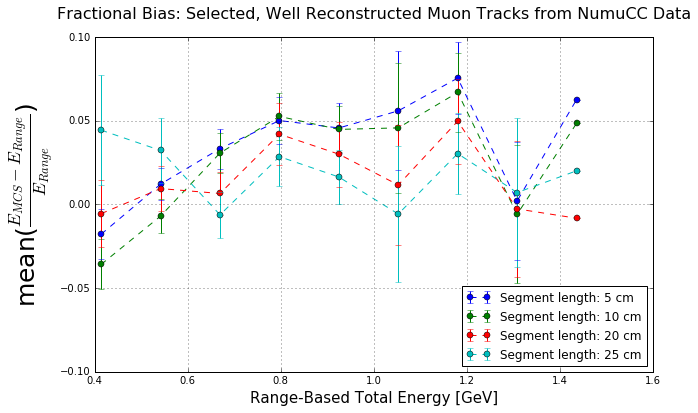
\includegraphics[width=75mm]{Figures/seglenstudy_DataRecoTracks_bias.png}}
	\quad
	\subfigure[\textit{MCS energy resolution as a function of range energy for four different segment lengths.}]
	{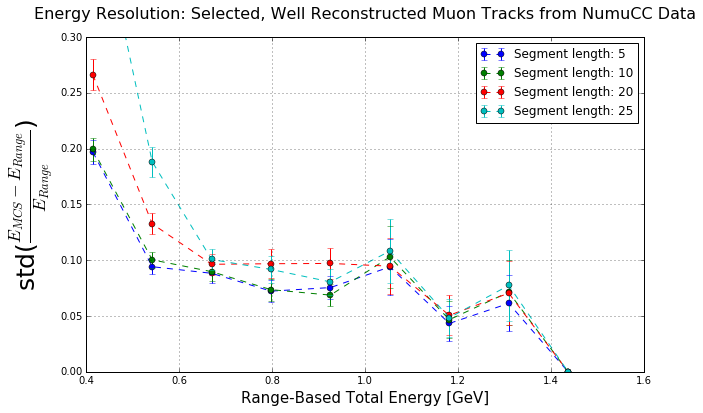
\includegraphics[width=75mm]{Figures/seglenstudy_DataRecoTracks_resolution.png}}
	}
\caption{\textit{MCS energy bias and resolution as a function of range energy for the selected, well reconstructed neutrino-induced muons in {\ub} data.}}
\label{seglenstudy_bias_resolution_DataRecoTrack_fig}
\end{figure}





\subsection{MCS to Determine Track Direction}\label{TrackDirection_DataRecoTrack_section}
This section demonstrates the ability for the multiple coloumb scattering code to determine the direction of a track. The MCS code as it is described in Section XXX works by maximizing a likelihood based on angular scatters between segments of a track along with the expected RMS angular deviation from the Highland equation (Equation \ref{highland_eqtn}) and assuming minimally ionizing energy loss in upstream portions of the track, since tracks tend to scatter more as they lose energy. In practice, there is actually a negative log likelihood that is minimized, meaning the lower the likelihood the more confident the fit is. In order to determine the direction of a track with MCS, one can compute the converged minimum log likelihood for the track assuming it is in the correct direction, then reverse the ordering of the trajectory points in the track and compute the converged minimum log likelihood for this ``backwards'' track. The likelihood should be better (smaller) for tracks in the correct direction than reversed tracks.\\

Given this sample in {\ub} data, the true direction of the track is known because it begins at the visible neutrino vertex. The minimized log likelihood for each of these tracks both in the correct (forwards) direction and incorrect (backwards) direction can be seen in Figure \ref{TrackDirection_DataRecoTrack_LLHDoverlay_fig}. A smaller likelihood here means a better fit in the MCS code. Figure \ref{TrackDirection_DataRecoTrack_LLHDdiff_fig} shows the difference of these two distributions, forwards minus backwards. Any negative entries in this figure indicate that the forwards-going track had a better fit than backwards-going. This figure shows that MCS can be used as a tool to test track direction in {\ub} data.

\begin{figure}
\centering
\mbox{
	\subfigure[\textit{The minimized log likelihood value for each track in the well-reconstructed, fully contained neutrino-induced muon tracks in data sample, both with tracks oriented in the correct (forwards) direction and reversed (backwards) direction. A smaller likelihood here means a better fit in the MCS code.}\label{TrackDirection_DataRecoTrack_LLHDoverlay_fig}]
	{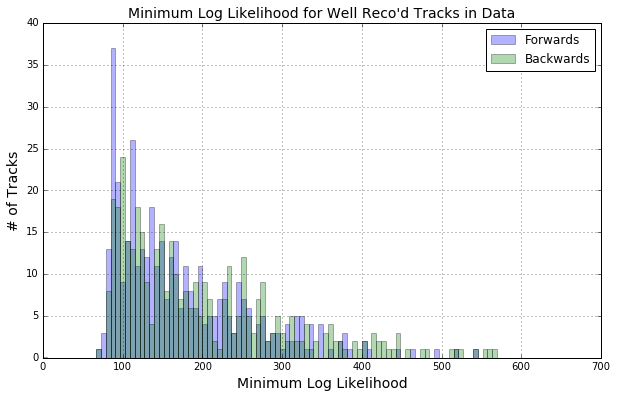
\includegraphics[width=75mm]{Figures/TrackDirection_DataRecoTrack_LLHDoverlay.png}}
	\quad
	\subfigure[\textit{The difference, forwards minus backwards, of the log likelihoods. Negative entries indicate that the forwards-going tracks had a better fit than the backwards-going ones.}\label{TrackDirection_DataRecoTrack_LLHDdiff_fig}]
	{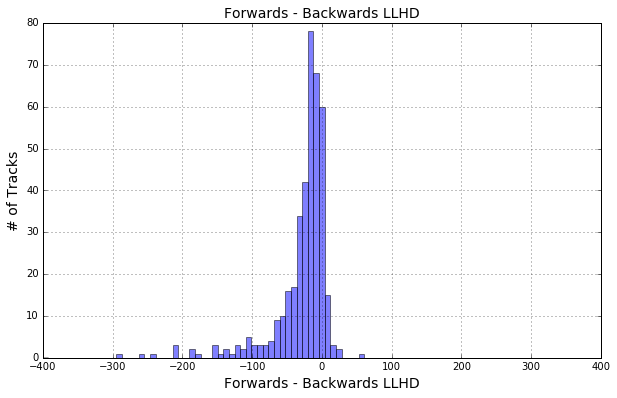
\includegraphics[width=75mm]{Figures/TrackDirection_DataRecoTrack_LLHDdiff.png}}
	}
\caption{\textit{Evidence that MCS can be used to determine track directions by analyzing the output of the likelihood fit.}}
\end{figure}